\documentclass{article}
\usepackage[top=2cm,bottom=2cm,left=3cm,right=3cm]{geometry}
\usepackage{hyperref}
\usepackage[utf8]{vietnam}
\usepackage{minted}
\usepackage{enumitem}
\usepackage{booktabs}
\usepackage{amssymb}
\usepackage{multirow}

\usepackage{tikz}
\usetikzlibrary{arrows.meta}
\usetikzlibrary{trees}
\usetikzlibrary{positioning}

\renewcommand{\familydefault}{\sfdefault}
\setlist[itemize]{topsep=0pt,itemsep=0pt}
\setlist[enumerate]{topsep=0pt,itemsep=0pt}

\title{\bf Kiểm thử luồng dữ liệu $-$ 2021II INT3117 1}
\author{Ngô Quang Dương/17020191}
\date{\today}

\begin{document}

\maketitle

\section{Chương trình đăng nhập}

\href{https://github.com/duong755/INT3117_1_2021II}{GitHub Repo}

\begin{minted}[linenos,frame=single,framesep=10pt,breaklines]{js}
var signInForm = document.forms[0];
signInForm.addEventListener('submit', function (submitEvent) {
  submitEvent.preventDefault();
  var email = document.querySelector('.text-field.email input').value;
  var emailErrorMessageContainer = document.querySelector('.text-field.email .error-message');
  var password = document.querySelector('.text-field.password input').value;
  var passwordErrorMessageContainer = document.querySelector('.text-field.password .error-message');
  var emailError = '';
  var passwordError = '';
  if (email.trim() === '') {
    emailError = 'Không được để trống email';
  } else if (!EMAIL_REGEX.test(email)) {
    emailError = 'Email không hợp lệ';
  } else if (email.trim().length > 320) {
    emailError = 'Email không được dài quá 320 kí tự';
  } else {
    emailError = '';
  }
  if (password.trim() === '') {
    passwordError = 'Không được để trống mật khẩu';
  } else {
    passwordError = '';
  }
  emailErrorMessageContainer.innerHTML = emailError;
  passwordErrorMessageContainer.innerHTML = passwordError;
  if (emailError === '' && passwordError === '') {
    this.submit();
  }
});
\end{minted}

\section{Các biến trong chương trình}

\par Chương trình trên sử dụng các biến sau (ở đây không nêu ra biến toàn cục \texttt{document}):

\begin{table}[htp]
    \centering
    % chktex-file 44
    \begin{tabular}{l|c|c|c}
        \texttt{Variable}                      & def                      & p-use            & c-use         \\
        \toprule
        \bottomrule
    \end{tabular}
    \caption{Bảng các biến và các dòng sử dụng chúng}
\end{table}

\begin{figure}[htp]
    \centering
    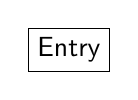
\begin{tikzpicture}[
            every node/.style={rectangle,draw},
            level 1/.style={level distance=1cm},
            level 3/.style={sibling distance=3cm}
        ]
        \tikzset{>=latex}
        \tikzset{edge from parent/.style={draw,-latex}}
        \node (entry node) {Entry};
    \end{tikzpicture}
    \caption{Đồ thị luồng dữ liệu}
\end{figure}

\section{Kiểm thử}

\subsection*{Path}

\par Dựa vào đồ thị luồng dữ liệu, ta xác định được 16 đường đi có thể có như sau:
\bigskip

\begin{enumerate}[label = (Path \arabic*),itemindent=1cm]
    \item 
    \item 
    \item 
    \item 
    \item 
    \item 
    \item 
    \item 
    \item 
    \item 
    \item 
    \item 
    \item 
    \item 
    \item 
    \item 
\end{enumerate}

\subsection*{def-clear path}

\begin{table}[htp]
    \centering
    % chktex-file 44
    \begin{tabular}{l|c|c}
        \texttt{Variable}                      & \texttt{def-clear path}                          & \texttt{path}                  \\
        \toprule
        \bottomrule
    \end{tabular}
\end{table}


\end{document}
